\section{Question 1}

\subsection{Question}
\verbatiminput{q1/q1.txt}

\subsection{Answer}
Using an example from the primary author of the D3 JavaScript library, Mike Bostok \cite{d3:bostok12}, a graph was created using Zachary's Karate Club as the dataset. The edge weights were obtained from the pickled \cite{py:pickle} dataset found at \url{http://nexus.igraph.org/api/dataset_info?id=1&format=html}. The D3 library provides a force-directed graphing layout \cite{d3:force14}, which was used to display the graph and to allow for a transition from the initial graph, shown in Figure \ref{fig:init_graph}, to the graph after the split of the karate club, shown in Figure \ref{fig:split_graph}.

\begin{figure}[h!]
\centering
\fbox{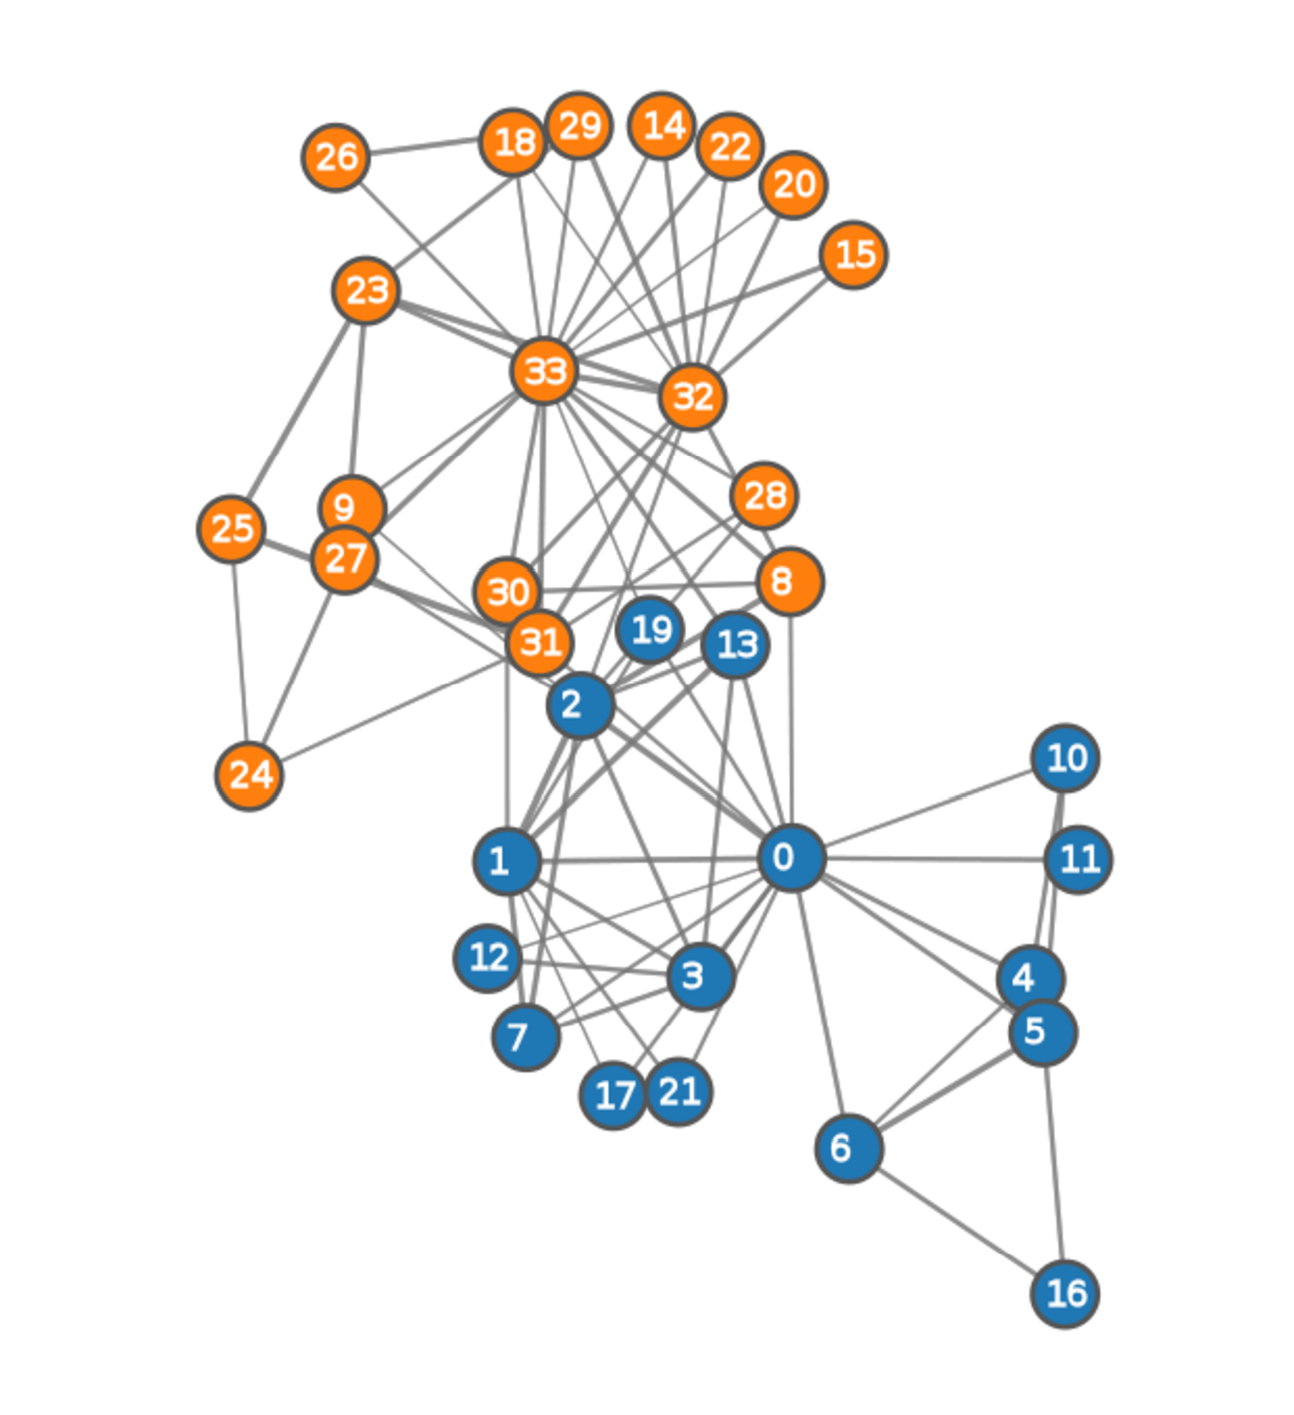
\includegraphics[scale=0.4]{q1/init_graph.pdf}}
\caption{Initial Graph}
\label{fig:init_graph}
\end{figure}

\begin{figure}[h!]
\centering
\fbox{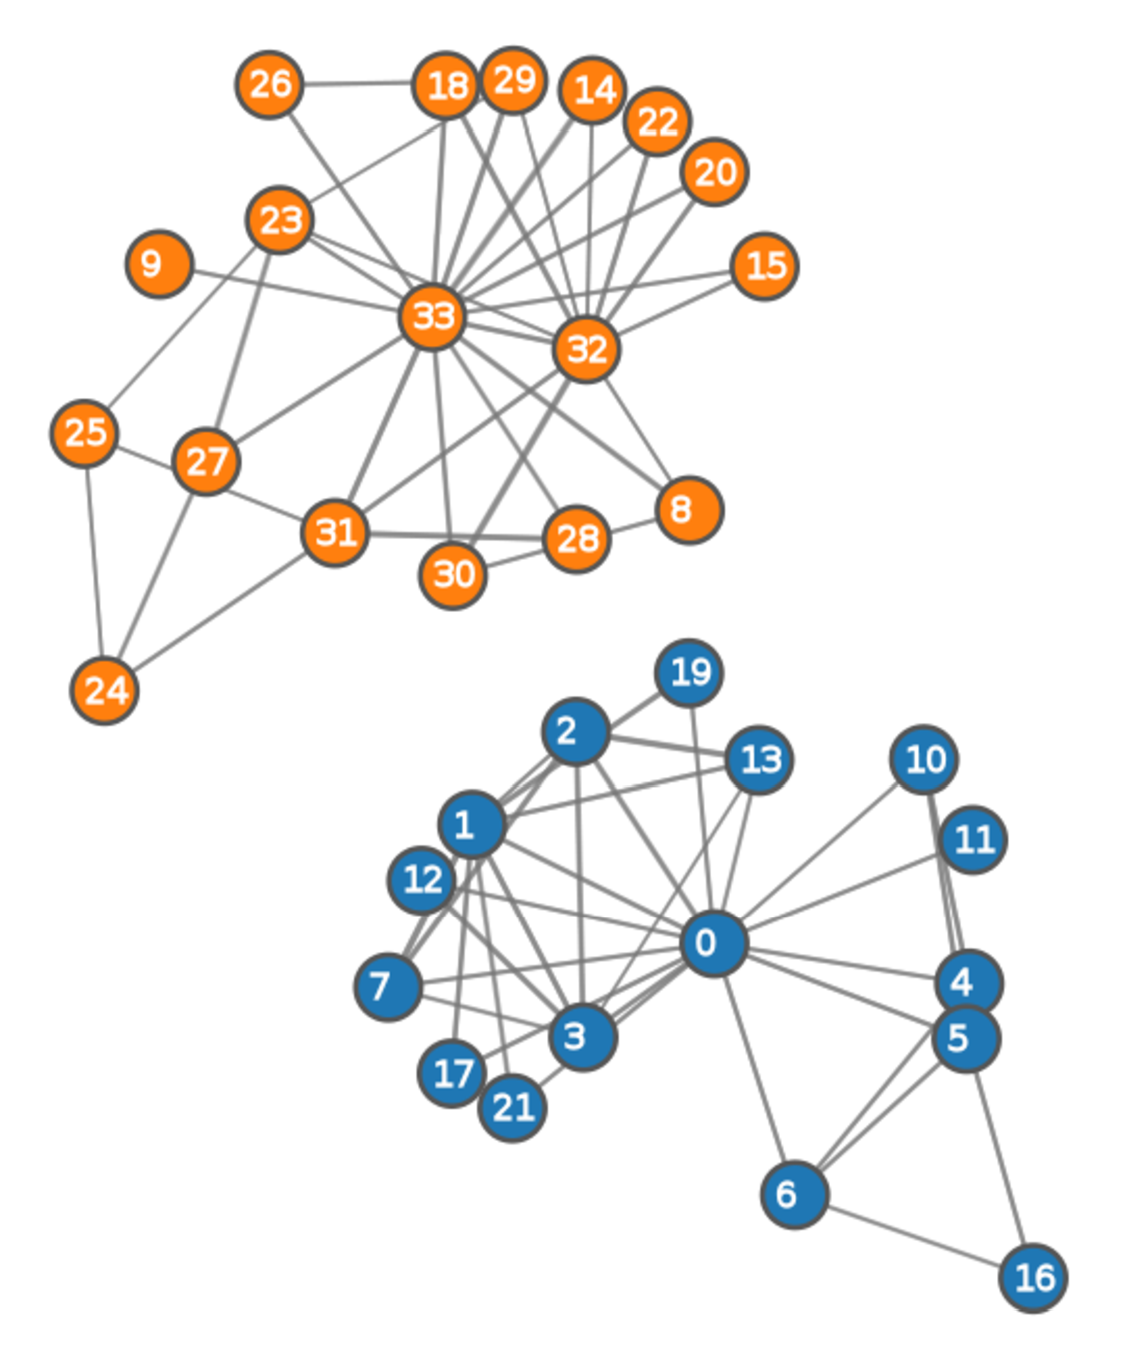
\includegraphics[scale=0.4]{q1/split_graph.pdf}}
\caption{Graph After Split}
\label{fig:split_graph}
\end{figure}

\clearpage

The dataset was first parsed into matrices using the {\tt build\_matrix} function, shown in Listing \ref{listing:convert}. These matrices were converted into python dictionary objects, which are pickled \cite{py:pickle} into the json format \cite{json}. This output was used as the input for the JavaScript code, which uses the D3 library \cite{d3} to create the graphs.

The python code to produce the json data is shown in Listing \ref{listing:convert}.

\lstinputlisting[language=Python, caption={Data Converter}, label=listing:convert]{q1/convert.py}

\clearpage

The javascript code to produce the graph is shown in Listing \ref{listing:build}.

\lstinputlisting[language=JavaScript, caption={Building the Graph}, label=listing:build,linerange={27-97},firstnumber=27]{q1/build_graph.html}
